
\section*{Extra slides}

\frame{
    \frametitle{Adapting the variance}
    \begin{figure}[tbp!]
    \begin{subfigure}[b]{0.49\textwidth}
        \centering
        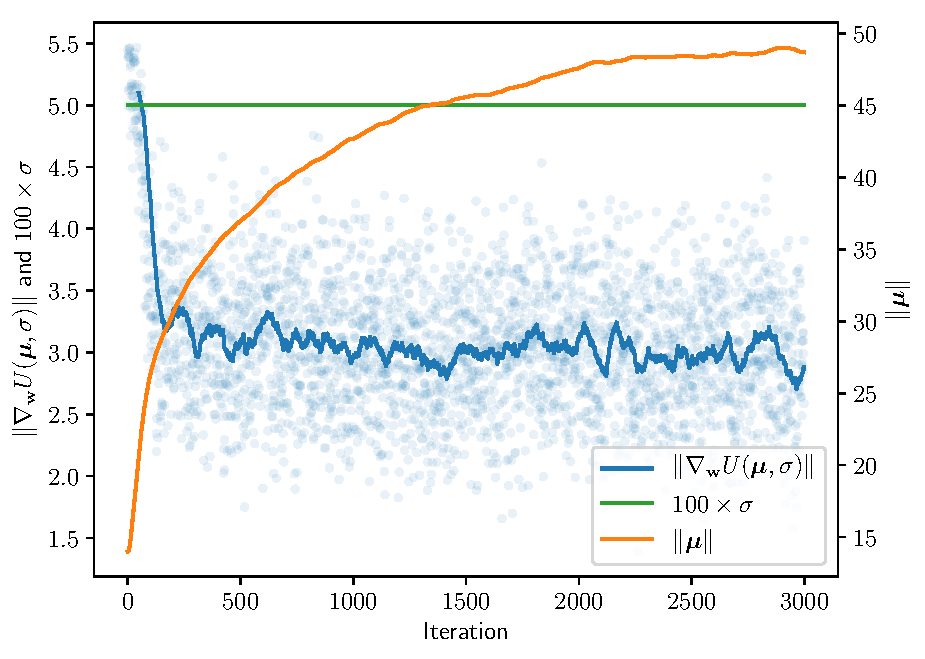
\includegraphics[height=4.2cm]{graphics/E031-NORM-analysis/isotropic-fixed-1-param-and-grad-and-variance-norm.pdf}
        \caption{}
        \label{fig: Theory: E031-NORM-analysis/isotropic-fixed-1-param-and-grad-and-variance-norm}
    \end{subfigure}
    \hfill
    \begin{subfigure}[b]{0.49\textwidth}
        \centering
        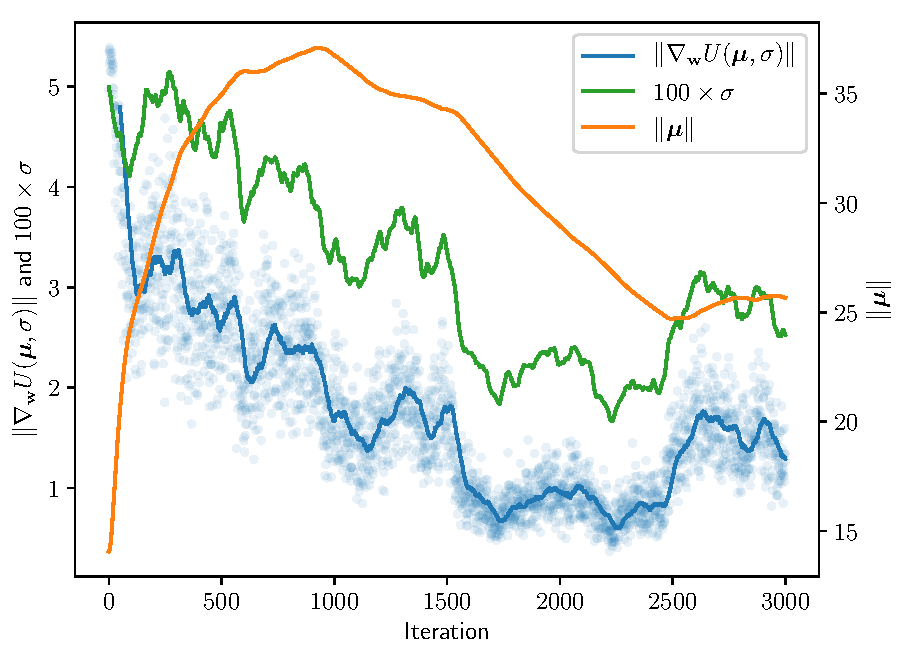
\includegraphics[height=4.2cm]{graphics/E031-NORM-analysis/isotropic-adapted-1-param-and-grad-and-variance-norm.pdf}
        \caption{}
        \label{fig: Theory: E031-NORM-analysis/isotropic-adapted-1-param-and-grad-and-variance-norm}
    \end{subfigure}
    \caption{
        2-norms of the \gls{NN} parameter vector and \gls{VO} gradient for an isotropic Gaussian search distribution with the variance overlayed (multiplied by 100 for scale). In \subref{fig: Theory: E031-NORM-analysis/isotropic-fixed-1-param-and-grad-and-variance-norm} and \subref{fig: Theory: E031-NORM-analysis/isotropic-adapted-1-param-and-grad-and-variance-norm}, the fixed and adapted variance versions are shown, respectively. A centered $50$ sample moving average is computed for the gradient. It is clear that adapting the variance directly and significantly influences the norm of the gradient and in turn also the norm of the parameter vector.
    }
    \label{fig: Theory: E031-NORM-analysis-isotropic}
\end{figure}
}

\frame{
    \frametitle{Adapting the variance}
    \begin{figure}[tbp!]
    \begin{subfigure}[b]{0.49\textwidth}
        \centering
        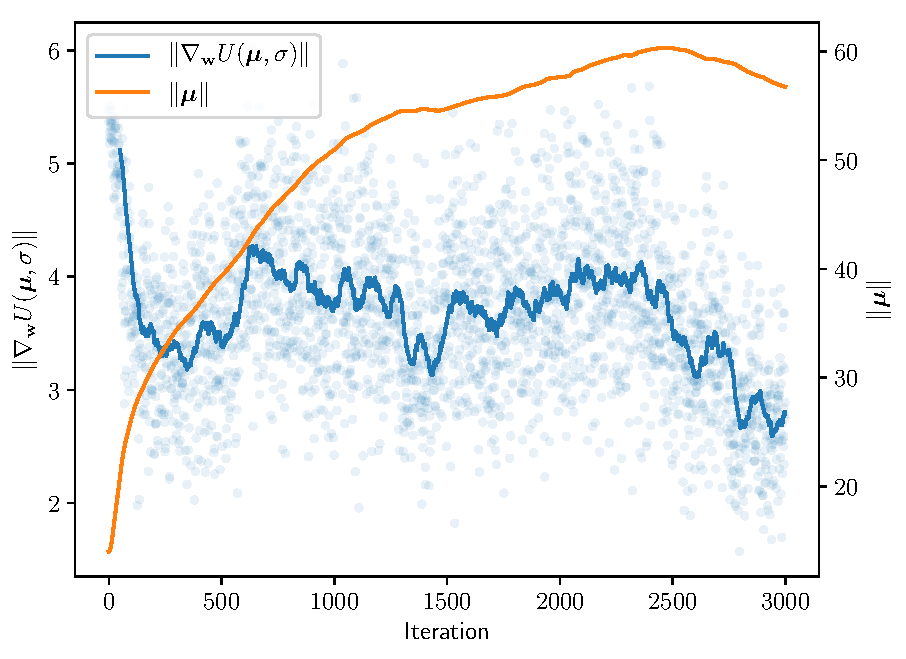
\includegraphics[height=4.4cm]{graphics/E031-NORM-analysis/separable-layer-5-param-and-grad-norm.pdf}
        \caption{}
        \label{fig: Theory: E031-NORM-analysis/separable-layer-5-param-and-grad-norm}
    \end{subfigure}
    \hfill
    \begin{subfigure}[b]{0.49\textwidth}
        \centering
        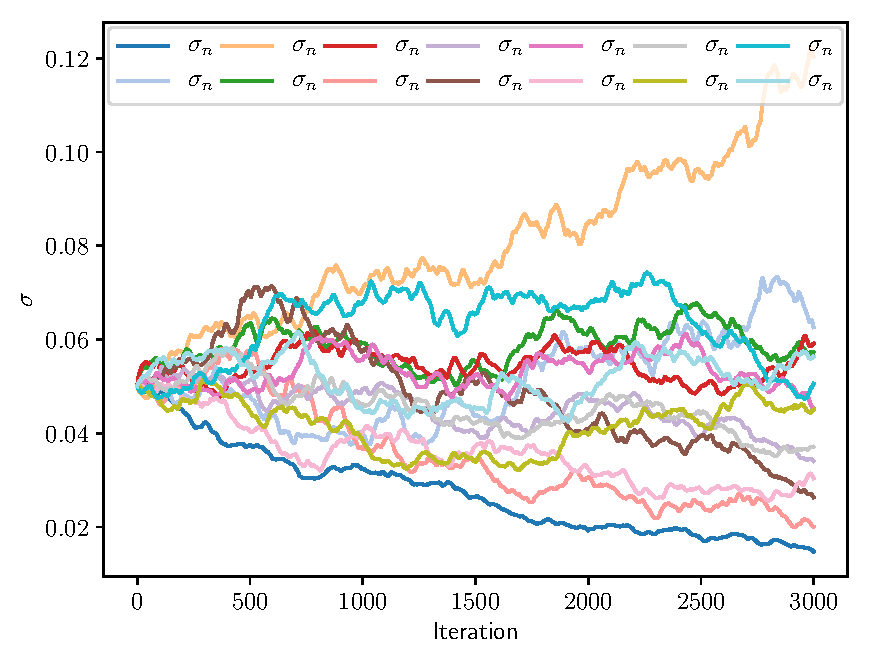
\includegraphics[height=4.4cm]{graphics/E031-NORM-analysis/separable-layer-5-variance.pdf}
        \caption{}
        \label{fig: Theory: E031-NORM-analysis/separable-layer-5-variance}
    \end{subfigure}
    \caption{
        \subref{fig: Theory: E031-NORM-analysis/separable-layer-5-param-and-grad-norm} 2-norms of the \gls{NN} parameter vector and \gls{VO} gradient for a layer-wise separable Gaussian search distribution with the variances plotted separately in \subref{fig: Theory: E031-NORM-analysis/separable-layer-5-variance}. Most variances tend to zero while a few increase. The gradient norm feels the combined effect but generally increases.
    }
    \label{fig: Theory: E031-NORM-analysis-layer-separable}
\end{figure}
}



\frame{
    \frametitle{Sensitivity rescaled perturbations}
    \begin{block}{Notation}
        \tabitem For a mini-batch of $I$ inputs $\X=\bmat{\x_1,\dots,\x_I}$ let $\Y(\X,\w) = NN(\X|\w)$\\
        \tabitem $Y_{ki}=NN(X_{:,i}|\w)_k$ equals value of $k$'th output unit for the $i$'th batch example
    \end{block}
    
    \begin{block}{Network divergence}
        \tabitem Divergence in network output units as result of additive perturbation $\epsilonb$
        \begin{equation}
            D(\epsilonb|\w) = \frac{1}{I}\sum_{k=1}^K\sum_{i=1}^I \pa{NN(\X|\w)_{ki} - NN(\X|\w+\epsilonb)_{ki}}^2
            \label{eq: Theory: Variational Optimization - Safe mutation divergence definition}
        \end{equation}
        \tabitem Perturbations that lead to large divergence risk \textbf{catastrophic forgetting}\\
    \end{block}
    \begin{block}{Rescaled perturbations}
        \tabitem Perturbations can be rescaled to correct for element-wise influence on divergence
        \begin{equation}
            \epsilonb_\text{safe} = \frac{\epsilonb}{\s}, \quad \epsilonb\sim p(\epsilonb|\thetab)
        \end{equation}
        with $\s$ computed in some appropriate way (line search, gradients)
    \end{block}
    
}

\frame{
    \frametitle{Sensitivity rescaled perturbations}
    \begin{block}{Network output gradients}
        \tabitem By Taylor expansion of outputs around $\w$, $\nabla_\w NN(\x_{i}|\w)_k$ can be seen as a point estimate of the sensitivity of the $k$'th output unit to changes in weights.
        \begin{equation}
        Y_{ki}(\epsilonb|\w) \approx NN(\x_{i}|\w)_k + \epsilonb\nabla_\w NN(\x_{i}|\w)
        \end{equation}
        \tabitem For a single output unit $k$, these can be averaged over a mini-batch of inputs
        \begin{equation*}
             \frac{1}{I}\sum_{i=1}^I \size{\nabla_\w NN(\X|\w)_{ki}} \quad \text{or} \quad \frac{1}{I}\sum_{i=1}^I \nabla_\w NN(\X|\w)_{ki}
        \end{equation*}
        \tabitem To handle the $K$ output units, the Euclidean length of the $K$ dimensional "vector" of sensitivities is taken to form $\s_\text{abs}$ or $\s_\text{sum}$, respectively
        \begin{equation}
            \sqrt{\sum_{k=1}^K \pa{\frac{1}{I}\sum_{i=1}^I\size{\nabla_\w NN(\X|\w)_{ki}}}^2} \quad \text{or} \quad \sqrt{\sum_{k=1}^K \pa{\sum_{i=1}^I\nabla_\w NN(\X|\w)_{ki}}^2}
        \end{equation}
        \tabitem $\s_\text{abs}$ is avoids gradient washout (absolute value) but $\s_\text{sum}$ is much more efficient
    \end{block}
    
    
}
